\input{../../../preamble.tex}


\begin{document}

    % \title{Математический анализ}
    % \date{26 сентября 2022}
    % \maketitle

    % \pagebreak

    % \subsection*{Определение интеграла Римана через интегральные суммы}
    {\noindent\large\textbf{Определение интеграла Римана через \hfill {\normalsize\boxed{\textbf{26 сентября 2022}}}\\интегральные суммы}} 

    $\Pi \subset \R^n, \ f : \Pi \rightarrow \R$ огр.
    \par $p$ -- разбиение $\Pi$, $= \{\pi_i, \ i = 1, \dots, N\}$
    \par $\Xi = \{\xi_i \in \pi_i, \ | \ i = 1, \dots, N\}$
    \par $\sum(f, p, \Xi) := \sum_{i=1}^N f(\xi) v(\pi_i)$ -- интегральная сумма Римана

    \begin{definition}
        Если $\exists I \in \R : \forall \{p_k\}_{k=1}^\infty : d(p_k) \xrightarrow[k \rightarrow]{} 0 \ \forall \{\Xi\}_{k=1}^\infty$
        \[
            \sum(f, p_k, \Xi_k) \xrightarrow[k \rightarrow \infty]{} I, \ \text{ то } f \text{ интегрируема по Риману и } I = \rhimani \Pi    
        \]
    \end{definition}

    \begin{theorem}
        $ $
        \par $\exists I \ \forall \{p_k\} : d(p_k) \xrightarrow[k \rightarrow \infty]{} 0 \ \forall \{\Xi\} \ \sum(f, p_k, \Xi_k) \xrightarrow[k \rightarrow \infty]{} I \Leftrightarrow \lrhimani \Pi = \urhimani \Pi = \rhimani \Pi$
    \end{theorem}
    
    \begin{proof}
        $ $
        \begin{enumerate}
            \item[$\boxed{\Rightarrow}$] $\epsilon, p_k : d(p_k) \xrightarrow[k \rightarrow \infty]{} 0 \ \forall \pi \in p_k \ \exists \xi \in \pi:$
                \[
                    f(\xi) - \inf_\pi f < \epsilon
                \]
                Получим $\Xi_k \ \sum(f, p_K, \Xi_k) - L(f, p_k) = \sum_{\pi \in p_k}(f(\xi(\pi)) - \inf_\pi f) \cdot v(\pi) <$
                \par \quad $< \epsilon \cdot \sum_{\pi \in p} v(\pi) = \epsilon \cdot v(\pi)$
                \par По \textit{Л. 3} $L(f, p_k) \xrightarrow[k \rightarrow \infty]{} \lrhimani \Pi \Rightarrow 0 \le I - \lrhimani \Pi \le \epsilon \cdot v(\pi)$
                \[
                    \begin{rcases}
                        \forall \epsilon \Rightarrow \lrhimani \Pi = I \\
                        \text{Аналогично } \urhimani \Pi = I
                    \end{rcases} \Rightarrow \exists \rhimani \Pi = I
                \]
            \item[$\boxed{\Leftarrow}$] Пусть $\lrhimani \Pi = \urhimani \Pi = \rhimani \Pi$. Возьмем произвольные
                \[
                    \{p_k\}, \ d(p_k) \rightarrow 0, \ \{\Xi_k\} \quad _{(*)}:    
                \]
                \[
                    L(f, p_k) \le \sum(f, p_k, \Xi_k) = \sum_{\pi \in p_k}\underbrace{f(\xi(\pi))}_{(*)} v(\pi) \le U(f, p_k)    
                \]
                \[
                    _{(*)} \quad \inf_\pi \le \dots \le \sup_\pi f    
                \]
                \[
                    L(f, p_k) \xrightarrow[\text{Л. 3, } k \rightarrow \infty]{} \lrhimani \Pi = \urhimani \Pi \xleftarrow[\text{Л. 3, } k \rightarrow \infty]{} U(f, p_k)    
                \]
                \[
                    \Rightarrow \sum(f, p_k, \Xi_k) \xrightarrow[k \rightarrow \infty]{} I
                \]
        \end{enumerate}
    \end{proof}

    \subsection*{Множество меры ноль}

    \begin{definition}
        $E \subset \R^n$ имеет меру ноль, если $\forall \epsilon > 0 \ \exists$ покрытие $E \subset \bigcup_{k = 1}^\infty C_k$, где $C_k$ -- открытые кубы
        \[
            \sum_{k=1}^\infty v(C_k) \le \epsilon \quad \quad \mu(E) = 0 \ \text{ -- мера}   
        \]
    \end{definition}

    \begin{remark}
        Открытые кубы $\Leftrightarrow$ замкнутые
    \end{remark}
    \begin{remark}
        $E_1 \subset E, \ \mu(E) = 0 \Rightarrow \mu(E_1) = 0$
    \end{remark}

    \begin{lemma}
        $\mu(E_k) = 0 \Rightarrow \forall k \in \N \Rightarrow \mu(\bigcup_{k=1}^\infty E_k) = 0$
    \end{lemma}

    \begin{proof}
        $\forall k \ \exists$ покрытие кубами с $\sum$ объемов $ < \epsilon \cdot (\frac{1}{2})^k$
        \par Тогда $E = \bigcup_{k=1}^\infty E_k$ будут покрыты и $\sum$ объемов $< \epsilon \cdot \sum_{k=1}^\infty (\frac 1 2)^k = \epsilon$
    \end{proof}

    \begin{definition}
        $E \subset \R^n$ имеет объем ноль, если $\forall \epsilon \ \exists$ конечное покрытие
        \par $E = \bigcup_{k=1}^\infty C_k$, где $c_k$ -- открытый куб
        \[
            \sum_{k=1}^N v(C_k) < \epsilon \quad \quad v(E) = 0   
        \]
    \end{definition}

    \begin{remark}
        $ $
        \begin{enumerate}
            \item открытые $\Leftrightarrow$ замкнутые кубы
            \item $v(E) = 0 \Rightarrow \mu(E) = 0$
        \end{enumerate}
    \end{remark}

    \begin{theorem}
        \par $[a, b] \subset \R$ не может иметь объем $0$
    \end{theorem}
    \begin{proof}
        докажем, что если $[a, b] \subset \bigcup_{k=1}^N C_k$,
        \[
            C_k \text{ -- отрезки, то } \sum_{k=1}^N v(C_k) \ge b - a
        \]
        база : $N = 1$
        \par \quad $[a, b] \subset C_1 \Rightarrow v(C_1) \ge b - a$
        
        \begin{figure}[H]

            \centering
            
            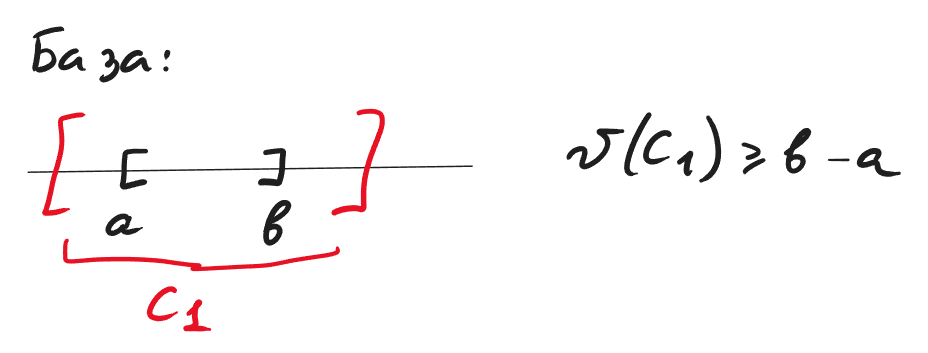
\includegraphics[width=0.8\linewidth]{База.png}
                   
        \end{figure}

        \par переход : $N + 1$
        \par \quad $a \in U_{k=1}^{N+1} C_k \Rightarrow \exists k : a \in C_k$ \text{ перенумеруем } $C_k$ так, чтобы $a \in C_1 = [\alpha, \beta]$
        \[
            \alpha \le a \le \beta \le b  
        \]

        \begin{figure}[H]

            \centering
            
            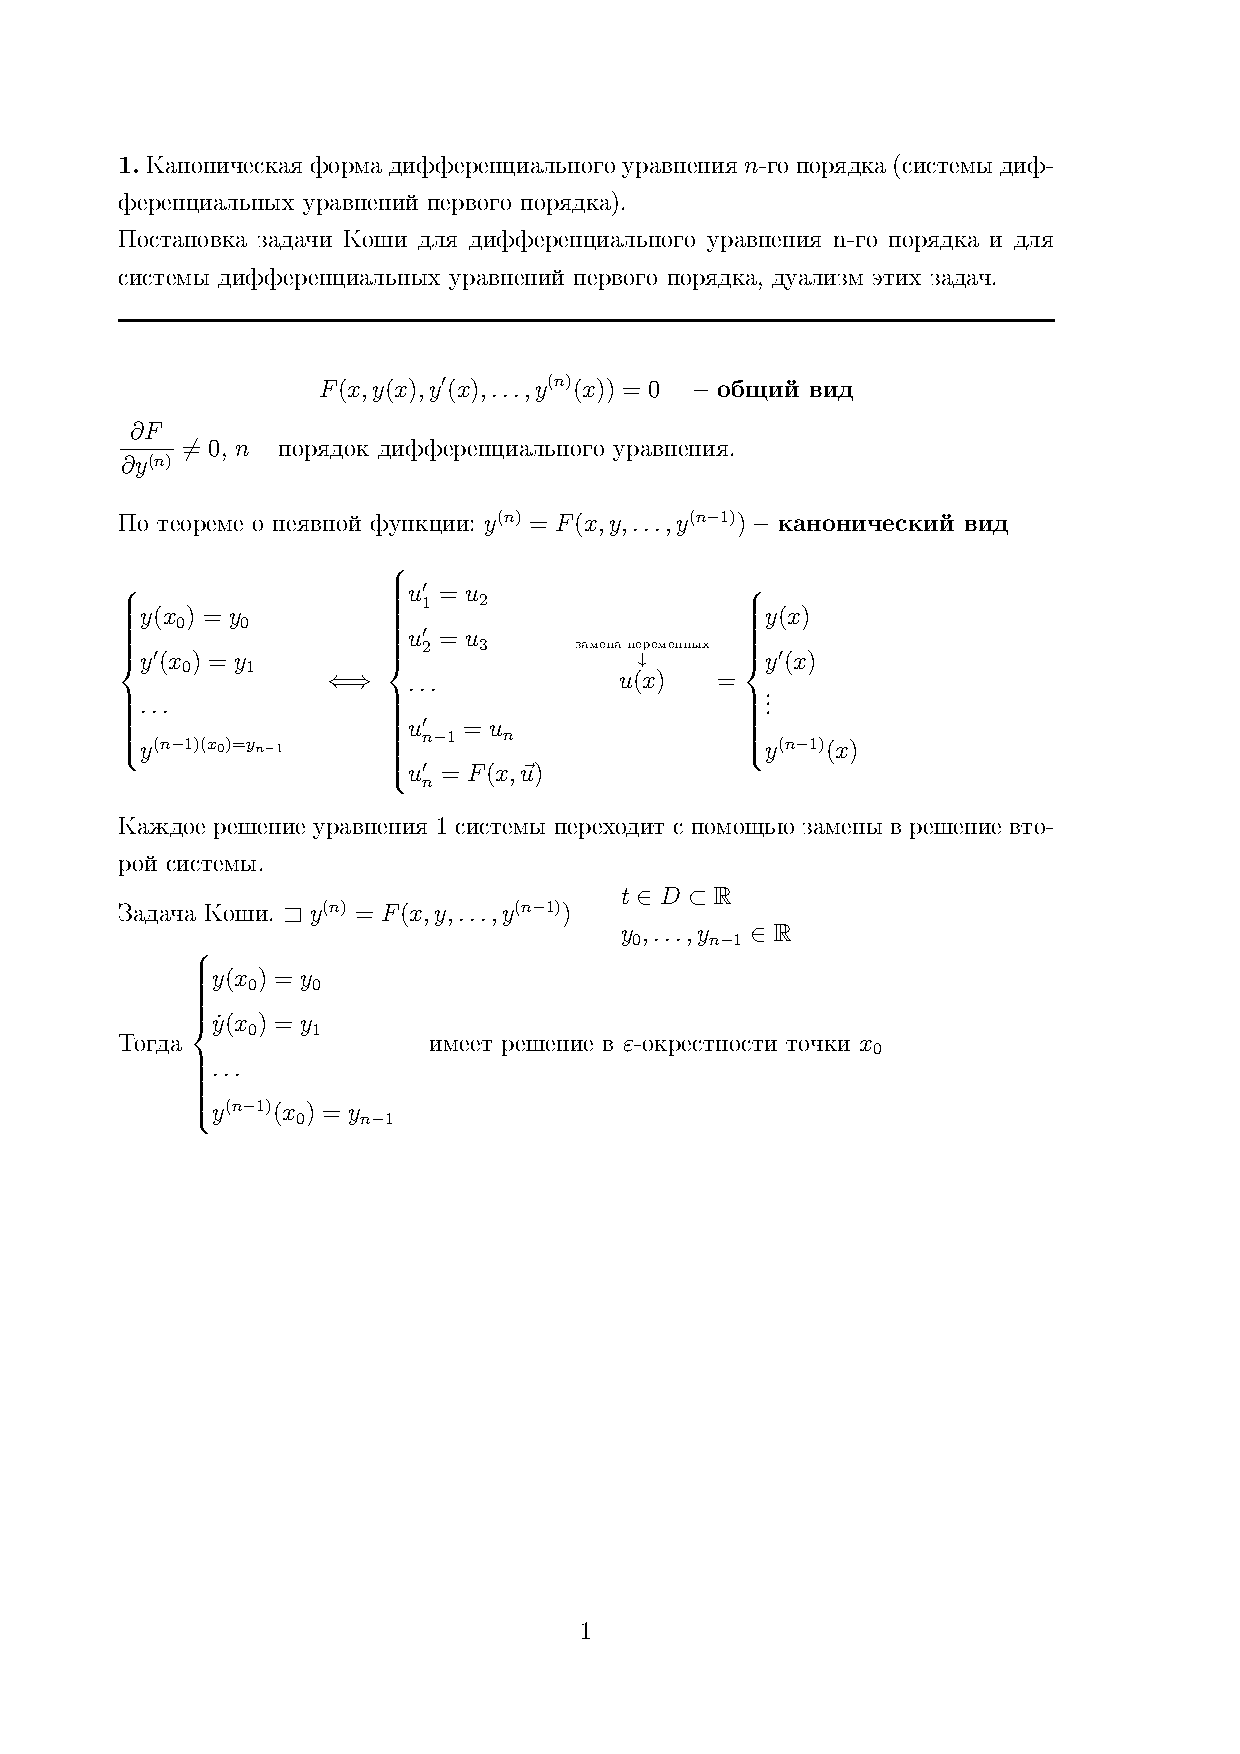
\includegraphics[width=0.8\linewidth]{1.png}
                   
        \end{figure}

        Если $b \in [\alpha, \beta]$, то $[a, b] \subset [\alpha, \beta]$,
        \[
            \sum_{k=1}^{N+1} v(C_k) > v(C_1) = \beta - \alpha \ge b - a    
        \]

        \begin{figure}[H]

            \centering
            
            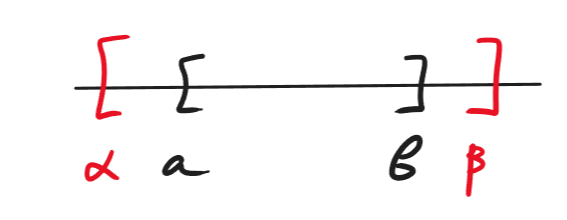
\includegraphics[width=0.8\linewidth]{2.png}
                   
        \end{figure}

        Если $b \not \in [\alpha, \beta], \ b > \beta$ 
        \[
            (\beta, b] \subset \bigcup_{k=2}^{N+1} C_k    
        \]
        \[
            \Rightarrow [\beta, b] \subset \bigcup_{k=2}^{N+1}  C_k \xRightarrow[\text{инд. п.}]{} \sum_{k=2}^{N+1} v(C_k) \ge b - \beta
        \]
        \[
            v(C_1) \ge \beta - a    
        \]
        \[
            \Rightarrow \sum_{k=1}^{N+1} v(C_k) \ge b - a    
        \]
    \end{proof}

    \begin{lemma}
        Если $K \subset \R^n$ компактно, то $v(K) = 0 \Leftrightarrow \mu (K) = 0$
    \end{lemma}
    \begin{proof}
        \begin{enumerate}
            \item[$\boxed{\Rightarrow}$] очев. (уже доказали)
            \item[$\boxed{\Leftarrow}$] Пусть $K \subset \bigcup_{k=1}^\infty C_k$ открытые кубы,
                \par $\sum_{k=1}^\infty v(C_k) < \epsilon$
                \par $\exists$ конечное подпокрытие $K \subset \bigcup_{j=1}^N C_{kj}$,
                \[
                    \sum_{j=1}^N v(C_{kj}) < \epsilon \Rightarrow v(K) = 0 
                \]
        \end{enumerate}
    \end{proof}

    \begin{illustration}
        $E = [0, 1] \cap \Q$ -- разные точки $\quad [a, b] = \{q_k, \ k \in \N\} = \bigcup_{k=1}^\infty \{q_k\}$
        \par $\mu(\{q_k\}) = 0 \ \forall k \xRightarrow[\text{Л. 4}]{} \mu(E) = 0$
        \par при этом $v(E) \not= 0$
        \par Пусть $E \subset \bigcup_{k=1}^N C_k \Rightarrow \underset{= [0, 1]}{\bar E} \subset \bigcup_{k=1}^N C_k \xRightarrow[\text{Л. 5}]{} \sum_{k=1}^N v(C_k) \ge 1$
    \end{illustration}

    \subsection*{Критерий интегрируемости Лебега}

    \textit{Почти везде} $\equiv$ везде, кроме множества точек, имеющего меру $0$
    \par $E \subset \R^n, \ f : E \rightarrow \R$ огранич.
    \par \quad $x \in \bar E, \quad \delta > 0$
    \par $M_\delta(f, x) := \sup_{B_\delta(x)} f, \quad m_\delta (f, x) := \inf_{B_\delta(x)} f$
    \par $M_\delta (f, x) \uparrow, \quad m_\delta (f, x) \downarrow$ - имеется в виду возрастание и убывание при росте $\delta$
    \par $M_\delta(f, x) - m_\delta(f, x) \ \uparrow$ по $\delta$ 
    


    \begin{definition}
        $\lim_{\delta \rightarrow 0^+} M_\delta(f, x) - m_\delta(f, x) = w(f, x)$ -- колеб. ф-ии $f$ в точке $x$
    \end{definition}

    \begin{lemma}
        $E \subset \R^n, \ f : E \rightarrow \R$ огр. \quad $x \in \bar E$
        \par $f$ непр. в точке $x \Leftrightarrow w(f, x) = 0$
    \end{lemma}
    \begin{proof}
        $ $

        \text{Расписать непрерывность на языке эпс-дельт, учесть монотонность колебания функции}

        \begin{enumerate}
            

            \item[$\boxed \Rightarrow$] $\forall \epsilon > 0 \ \exists \delta_\epsilon > 0 \ \forall y \in B_\delta(x) \cap E \ |f(x) - f(y)| < \epsilon$
                \par $\Rightarrow M_{\delta_\epsilon}(x) - m_{\delta_\epsilon}(x) \le \epsilon$
                \par и более того, $\forall \delta < \delta_\epsilon \ M_{\delta}(x) - m_{\delta}(x) < \epsilon$ \
                                \par $M_\delta(f, x) - m_\delta(f, x) \xrightarrow[\delta \rightarrow 0^+]{} 0$
                \par то есть $w(f, x) = 0$
            \item[$\boxed \Leftarrow$] $w(f, x) = 0 \Rightarrow \forall \epsilon \ \exists \delta_\epsilon : \forall \delta < \delta_\epsilon$
                \par $M_\delta(f, x) - m_\delta(f, x) < \epsilon$
                \par $\forall y \in B_\delta(x) \cap E \quad |f(y) - f(x)| < \epsilon$
                \par $f(y) \xrightarrow[y \rightarrow x]{} f(x)$
        \end{enumerate}


    \end{proof}

    \begin{lemma}
        $F \subset \R^n$ замкн., $f : F \rightarrow \R$ огр.
        \par $\forall \epsilon > 0 : F_\epsilon := \{x \in F \ | \ w(f, x) \ge \epsilon\}$. Т. д. $F_\epsilon$ -- замкн.
    \end{lemma}
    \begin{proof}
        Докажем, что $\R \setminus F_\epsilon$ -- откр.
        \[
            \begin{array}{c}
                1. \ x \in \R^n \setminus F \\
                2. \ x \in F \setminus F_\epsilon
            \end{array} \xRightarrow[]{??} \delta > 0 \quad B_\delta(x) \in \R^n \setminus F_\epsilon
        \]
        \begin{enumerate}
            \item $x \in \underbrace{\R^n \setminus F}_{\text{откр.}} \Rightarrow \exists \delta > 0 \ B_\delta(x) \subset \R^n \setminus F \subset \R^n \setminus F_\epsilon$
            \item $x \in F \setminus F_\epsilon \Rightarrow w(f, x) < \epsilon \Rightarrow \exists \delta > 0 : M_\delta(f, x) - m_\delta(f, x) < \epsilon$
                \[
                    y \in B_\delta(x) \ \exists \delta' > 0 \ B_{\delta'}(y) \subset B_\delta(y)    
                \]
                \[
                    (\delta' < \delta - \|x-y\|)    
                \]
                если $y \not\in F$, то $y \in \R^n \setminus F \subset \R^n \setminus F_\epsilon$
                \par если $y \in F$, то $w(f, y) < \epsilon$
                \[
                    M(f, \delta_1, y) - m(f, \delta_1, y) \le M(f, \delta, x) - m(f, \delta, x) < \epsilon
                \]
                 \[
                       \Rightarrow w(f, y) < \epsilon \Rightarrow y \in \R^n \setminus F_\epsilon
                 \]

                 Тогда $\forall y \in B_\delta(x)$ верно, что $y \not \in F_\epsilon$ или $B_\delta(x) \cap F_\epsilon = \emptyset$

                 $x \in F \setminus F_\epsilon$, $B_\delta(x)$ полностью лежит в $F \setminus F_\epsilon$, значит оно открыто, $F$ - замкнуто, $F \setminus (F \setminus F_\epsilon) = F_\epsilon$ - замкнуто
        \end{enumerate}
    \end{proof}

    \begin{lemma}
        $\Pi \subset \R^n, \ f : \Pi \rightarrow \R$ огр.
        \par Если $\forall x \in \Pi \quad w(f, x) < \epsilon$, то  $\exists$ разбиение $p$:
        \[
            U(f, p) - L(f, p) < \epsilon \cdot v(\Pi)    
        \]
    \end{lemma}
    \begin{proof}
        $\forall x \in \Pi \ \lim_{\delta \rightarrow 0^+}(M_\delta(f, x) - m_\delta(f, x)) = 0 $
        \par $\exists \delta_\epsilon : M_{\delta_\epsilon}(f, x) - m_{\delta_\epsilon}(f, x) < \epsilon$
        \par $\forall x \ \exists \pi_x$ открытый п/п : $\underline{\sup}_{\pi_x} f - \underline{\inf}_{\pi_x} f < \epsilon$
        \par $\Pi \subset \bigcup_{x \in \Pi} \pi_x$, $\Pi$ компактен $\Rightarrow \exists$ конечное подпокрытие
        \[
            \Pi \subset \bigcup_{k=1}^N \pi_{x_k}    
        \]
        разрешем $\Pi$ гранями всех $\pi_{x_k}, \ k = 1, \dots, N$
        \par $\Rightarrow$ получаем разбиение $p$
        \[
            U(f, p) - L(f, p) = \sum_{\pi \in p} (\sup_\pi f - \inf_\pi f) v(\pi) < \epsilon \cdot \sum_{\pi \in p} v(\pi) = \epsilon v(\pi)    
        \]
        \[
            \forall \pi \in p \ \exists k \ \pi \subset \bar \pi_{x_k}    
        \]
        \[
            \Rightarrow \sup_\pi f - \inf_\pi f \le \sup_{\bar \pi_{x_k}} f - \inf_{\bar \pi_{x_k}} f < \epsilon
        \]
    \end{proof}

    \begin{theorem}
        Критерий Лебега    

        \par $\Pi \in \R^n$ - п/п $f: \Pi \rightarrow \R$ - огр 
        \par $D = \{x \in \Pi | f - \text{разрывна в x}\}$
        \par Тогда:
        $$\exists \rhimani \Pi f \Leftrightarrow \mu(D)=0$$
    \end{theorem}

    \begin{proof}
        \par Пусть $\Pi_\epsilon = \{x \in \Pi | w(f,x) \ge \epsilon \}$ - замкнутые по Лемме, ограниченные из ограниченности исходного п/п, значит компактные
        $$D \subset \bigcup_{\epsilon > 0} \Pi_\epsilon$$
        \bigskip
        \par $\boxed{\Leftarrow}$ $\mu(D) = 0$ 
        $$\mu(\Pi_\epsilon) = 0, \forall \epsilon>0 \Rightarrow v(\Pi_\epsilon) = 0$$
        $$\Pi_\epsilon \subset \bigcup\limits_{k=1}^N \pi_k, \sum\limits_{k=1}^N < \epsilon, \pi_k \text {- открытые кубы}$$
        \par Разрежем $\Pi$ гранями $\pi_1 ... \pi_N$ - получим разбиение $P$
        \par $P = P_1 \cup P_2$, $P_1, P_2$ - не разбиения, но состоят из кубов
        \par $P_1 = \{\pi \in P | \exists k: \pi \in \overline{\pi_k} \}$
        \par $P_2 = P \setminus P_1$
        $$\sum\limits_{\pi \in P_1} v(\pi) \le \sum\limits_{k=1}^N v(\pi_k) < \epsilon$$
        \bigskip
        \par $f$ - огр, значит $\exists M>0: \forall x \in \Pi |f(x)| < M$
        $$\sum\limits_{\pi \in P_1} (M_\pi(f) - m_\pi(f)) \cdot v(\pi) \le 2M \cdot \sum\limits_{\pi \in P_1} v(\pi) \le 2M \cdot \epsilon$$
        \bigskip
        \par $\forall \pi \in P_2: \forall x\in \pi: w(f, x) < \epsilon$
        $$\exists P(\pi): U(f, P(\pi)) - L(f, P(\pi)) < \epsilon \cdot v(\pi)$$
        \par Разрежем $\Pi$ гранями $\pi' \in P(\pi)$ для всех $\pi \in P_2$
        \par Получим разбиение $\Pi$: $P' = P_1' \cup P_2'$, $P_1', P_2'$ - более мелкие по сравнению с $P_1, P_2$
        $$\sum\limits_{\pi' \in P_1'} (sup_{\pi'} f - inf_{\pi'} f)v(\pi') \le 2M \cdot \sum\limits_{\pi' \in P_1'} v(\pi') < 2M \cdot \epsilon$$
        \bigskip
        $$\sum\limits_{\pi' \in P_2'} (sup_{\pi'} f - inf_{\pi'} f)v(\pi') = \sum\limits_{\pi \in P_2} \sum\limits_{\pi' \in P(\pi)} (sup_{\pi'} f - inf_{\pi'} f)v(\pi') < \sum\limits_{\pi \in P_2} \epsilon \cdot v(\pi) < \epsilon \cdot v(\Pi)$$
        \bigskip
        $$U(f, P') - L(f, P') = \sum\limits_{\pi' \in P'} (sup_{\pi'} f - inf_{\pi'} f) v(\pi') < \epsilon \cdot (2M + v(\Pi)) \Rightarrow \exists \rhimani \Pi f$$
        \bigskip
        \par $\boxed{\Rightarrow}$ $\exists \rhimani \Pi f$
        \par Хотим доказать, что $\mu(D) = 0$
        $$D = \bigcup\limits_{k=1}^{\infty} \Pi_{1/k}$$
        \par Если $\forall k: \mu(\Pi_{1/k}) = 0$, то по лемме о мере счётного объединения множеств меры 0 докажем необходимое
        \bigskip
        \par Из существования интеграла: $\forall \epsilon>0 \exists P: U(f, P) - L(f, P) < \frac{\epsilon}{k}$
        $$P_k = \{\pi \in P | \Int \pi \cap \Pi_{1/k} \not = \emptyset \}$$
        $$\Pi_{1/k} \subset \bigcup\limits_{\pi \in P_k} \pi$$
        $$\forall \pi \in P_k \ \exists x \in \Int \pi: w(f, x) \ge \frac{1}{k}$$
        $$\exists \delta > 0: B_{\delta}(x) \in \Int  \pi \ sup_{B_{\delta}(x)} f - inf_{B_{\delta}(x)} f \ge \frac{1}{k}$$
        $$sup_{\pi} - inf_{\pi} \ge sup_{B_{\delta}(x)} f - inf_{B_{\delta}(x)} f \ge\frac{1}{k}$$
        \bigskip
        $$U(f, P) - L(f, P) = \sum\limits_{\pi \in P} (sup_{\pi} f - inf_{\pi} f) v(\pi) \ge \sum\limits_{\pi \in P_k} (sup_{\pi} f - inf_{\pi} f) v(\pi) \ge \frac{1}{k} \cdot \sum\limits_{\pi \in P_k} v(\pi)$$
        $$\sum\limits_{\pi \in P_k} v(\pi) \le k \cdot (U(f, P) - L(f, P)) < \epsilon$$
        \bigskip
        $$v(\Pi_{1/k}) = 0$$ 



    \end{proof}


\end{document}